%%%%%%%%%%%%%%%%%%%%%%%%%%%%%%%%%%%%%%%%%
% Stylish Article
% LaTeX Template
% Version 2.1 (1/10/15)
%
% This template has been downloaded from:
% http://www.LaTeXTemplates.com
%
% Original author:
% Mathias Legrand (legrand.mathias@gmail.com) 
% With extensive modifications by:
% Vel (vel@latextemplates.com)
%
% License:
% CC BY-NC-SA 3.0 (http://creativecommons.org/licenses/by-nc-sa/3.0/)
%
%%%%%%%%%%%%%%%%%%%%%%%%%%%%%%%%%%%%%%%%%

%----------------------------------------------------------------------------------------
%	PACKAGES AND OTHER DOCUMENT CONFIGURATIONS
%----------------------------------------------------------------------------------------

\documentclass[fleqn,10pt]{SelfArx} % Document font size and equations flushed left

\usepackage[italian]{babel} % Specify a different language here - english by default

\usepackage{float}
%----------------------------------------------------------------------------------------
%	COLUMNS
%----------------------------------------------------------------------------------------

\setlength{\columnsep}{0.55cm} % Distance between the two columns of text
\setlength{\fboxrule}{0.75pt} % Width of the border around the abstract

%----------------------------------------------------------------------------------------
%	COLORS
%----------------------------------------------------------------------------------------

\definecolor{color1}{RGB}{0,0,90} % Color of the article title and sections
\definecolor{color2}{RGB}{0,20,20} % Color of the boxes behind the abstract and headings

%----------------------------------------------------------------------------------------
%	HYPERLINKS
%----------------------------------------------------------------------------------------

\usepackage{hyperref} % Required for hyperlinks
\hypersetup{hidelinks,colorlinks,breaklinks=true,urlcolor=color2,citecolor=color1,linkcolor=color1,bookmarksopen=false,pdftitle={Title},pdfauthor={Author}}

%----------------------------------------------------------------------------------------
%	ARTICLE INFORMATION
%----------------------------------------------------------------------------------------

\JournalInfo{Progetto del corso \textit{Industry Lab}, Università degli Studi di Milano Bicocca} % Journal information
\Archive{Anno Accademico 2019-20} % Additional notes (e.g. copyright, DOI, review/research article)

\PaperTitle{GP5 - Analisi dei dati e previsione del coefficiente di perdita} % Article title

\Authors{Riccardo Cervero\textsuperscript{1}, Marco Savino\textsuperscript{2}, Luca Lazzati\textsuperscript{3}} % Authors
\affiliation{\textsuperscript{1}\textit{794126, Dipartimento di Informatica, Sistemistica e Comunicazione}} % Author affiliation
\affiliation{\textsuperscript{2}\textit{793516, Dipartimento di Informatica, Sistemistica e Comunicazione}} % Author affiliation
\affiliation{\textsuperscript{3}\textit{?, Dipartimento di Informatica, Sistemistica e Comunicazione}}

\Keywords{Monitoraggio -- Previsione} % Keywords - if you don't want any simply remove all the text between the curly brackets
\newcommand{\keywordname}{Keywords} % Defines the keywords heading name

%----------------------------------------------------------------------------------------
%	ABSTRACT
%----------------------------------------------------------------------------------------

\Abstract{}

%----------------------------------------------------------------------------------------

\begin{document}

\flushbottom % Makes all text pages the same height

\maketitle % Print the title and abstract box

\tableofcontents % Print the contents section

\thispagestyle{empty} % Removes page numbering from the first page

%----------------------------------------------------------------------------------------
%	ARTICLE CONTENTS
%----------------------------------------------------------------------------------------

\section*{Caso di studio} % The \section*{} command stops section numbering

\addcontentsline{toc}{section}{Caso di studio} 

%Spiegazione problema

%------------------------------------------------
\section{Data Preparation}
Il \textit{database} si compone di 296605 osservazioni, descritte da 33 colonne. Tuttavia, è stato necessario focalizzare l'analisi su quelle che presentavano un certo grado di rilevanza e utilità per l'oggetto di studio. Ciò ha comportato la rimozione, durante una prima fase di \textit{pre-processing}, delle variabili che presentavano le seguenti caratteristiche: si manifestavano come un unico valore costante\footnote{Le costanti rimosse sono: \texttt{"Banco"}, \texttt{"Master"}, \texttt{"Picco coppia zero"}, \texttt{"Picco coppia iniziale"}, \texttt{"Media coppia iniziale"}, \texttt{"Velocità 1"}, \texttt{"Picco pressione velocità 2"}, \texttt{"Media pressione velocita 2"}, \texttt{"Picco portata velocità 2"}, \texttt{"Media portata velocità 2"}.}, mostravano una distribuzione eccessivamente sbilanciata verso una sola classe\footnote{È questo il caso di \texttt{"Velocità 2"}, \texttt{"Esito"} e di conseguenza \texttt{"N. Esito"}, \texttt{"Coppia max ciclo"}, \texttt{"Velocità a regime"}.}, erano ridondanti, poco interessanti o erano già state segnalate tali dai fornitori del \textit{dataset}\footnote{Le colonne inutili sono: \texttt{"Codice da Linea"} - identificativo del pezzo -, \texttt{"Media coppia zero"}, \texttt{'Data'} e \texttt{'Ora'}, poiché i dati sono stati raccolti in un arco temporale non uniforme.}.\\
Successivamente, è stata rimossa una riga, poiché penalizzata dalla mancanza dei valori di pressione. Infine, poiché la differenza di scala era spesso eccessiva per molte colonne numeriche, si è deciso di normalizzare la matrice originale, mappando tutte le variabili non categoriche fra 0 e 1. 
%------------------------------------------------
\section{Analisi preliminari}
Dopo le operazioni di pulizia appena menzionate, si è proceduto ad analizzare in maniera preliminare le colonne rilevanti, per ottenere un primo approfondimento sui descrittori e i rapporti di dipendenza fra gli stessi. 
\subsection{Variabili categoriche}
I dati nominali conservati sono relativi a due precisi aspetti del processo: la segmentazione del lavoro in turni differenti e il programma selezionato per la creazione del pezzo, ovvero la tiplogia di pompa.\\
Per quanto riguarda la prima, è stato necessario aggregare le medesime classi registrate erroneamente in maniera diversa, uniformandone la denominazione. In questo modo, sono state ottenute 5 classi: "A", "B", "C", "D", "0". Le ultime due, poiché osservate in minor misura e non specificate inizialmente dai fornitori del \textit{dataset}, sono state etichettate come \textit{missing values}.
\begin{figure}[h]
    \centering
    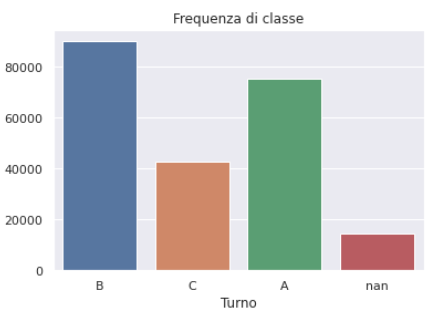
\includegraphics[width=0.9 \linewidth]{turno.png}
    \label{fig:em}
    \caption{\textit{Bar chart} per la visualizzazione delle rispettive frequenze osservate dei turni.}
\end{figure}
Come osservabile in Figura 1, i principali blocchi in cui è organizzato il processo presentano una frequenza diversa: il turno "B" costituisce più del 40\% dei \textit{records}, "A" si presenta nel $\sim$34\% dei casi e "C" nel $\sim$19\%.\\
La composizione del "Programma" mostra un fortissimo sbilanciamento verso la classe GP5 denominata \texttt{18\_GP5\_910\_CW} (Figura 2), che corrisponde alla pompa "\textit{Daimler}". Le restanti tipologie, raggruppate sotto denominazione "Standard", formano in totale meno del 23\% dei casi e sono principalmente rappresentate dalle categorie \texttt{17\_GP5\_430\_CCW} (10.6\%) e \texttt{12\_GP5\_430B\_D1} (8.5\%).
\begin{figure}[h]
    \centering
    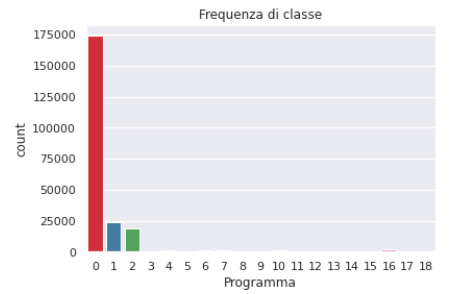
\includegraphics[width=0.9 \linewidth]{prog.png}
    \label{fig:em}
    \caption{\textit{Bar chart} per la visualizzazione delle rispettive frequenze osservate dei programmi.}
\end{figure}
Per una visualizzazione migliore, in Figura 3 è riassunta la distribuzione delle frequenze logaritmiche delle varie classi GP5.
\begin{figure}[h]
    \centering
    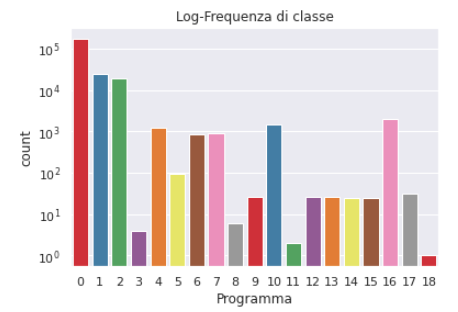
\includegraphics[width=0.9 \linewidth]{proglog.png}
    \label{fig:em}
    \caption{\textit{Bar chart} per la visualizzazione delle rispettive frequenze logaritmiche dei programmi.}
\end{figure}
\\
Tra le variabili categoriche esaminate, "Esito" descrive le eventuali - rarissime - imperfezioni del prodotto. A tal proposito, il 99.5\% delle volte il risultato è ottimale, mentre l'anomalia più comune è indicata come "scarto picco coppia max fase pulizia iniziale" (0.1\% delle osservazioni).
\subsection{Variabili numeriche}
I dati numerici registrano, per ogni pompa, due principali set di valori, relativi al picco e alla media di pressione (in bar) e portata (in litri all'ora), misurati in corrispondenza di due velocità diverse:
\begin{itemize}
    \item a regime: 2300 \textit{r.p.m}
    \item 140 \textit{r.p.m}
\end{itemize}
Si vedrà che, a prescindere dalla velocità, le due grandezze condividono un'elevatissima dipendenza lineare.
\subsubsection{Descrittori della pressione}
Innanzitutto, le grandezze relative al picco e alla media hanno una distribuzione multimodale nell'ambito di entrambe le misurazioni della velocità (Figura 4), rivelando picchi di diversa altezza. Il range osservato è molto superiore per quanto concerne la velocità a regime (come riassunto dalla Tabella 1). Inoltre, le distribuzioni dei valori appaiono quasi identiche per classe di velocità, rivelando una fortissima similarità fra l'andamento del picco e e della pressione media (Figura 5).
\begin{figure}[h]
    \centering
    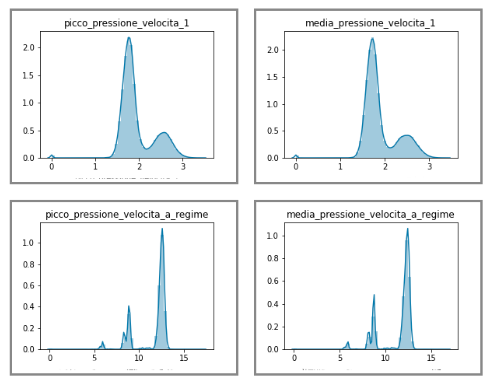
\includegraphics[width=1 \linewidth]{press.png}
    \label{fig:em}
    \caption{Distribuzioni delle grandezze relative alla pressione.}
\end{figure}
\begin{figure}[h]
    \centering
    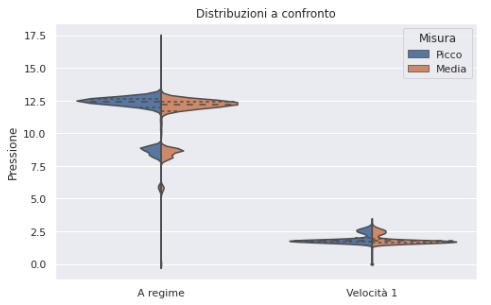
\includegraphics[width=1 \linewidth]{p.png}
    \label{fig:em}
    \caption{Distribuzioni delle grandezze relative alla pressione, in corrispondenza della velocità "1" e a regime, appaiate nell'ambito della stessa misurazione. È possibile notare sia la superiorità della pressione a regime, che la fortissima vicinanza dell'andamento del picco rispetto alla pressione media.}
\end{figure}
{\begin{table}[h]
\centering
\begin{tabular}[t]{lccc}
\toprule
Pressione&Minimo&Media&Massimo\\
\midrule
\textbf{Picco (140)}&0.19&1.94&3.45\\
\textbf{Picco (2300)}&5.38&11.61&14.21\\
\textbf{Media (140)}&0.1&1.88&3.38\\
\textbf{Media (2300)}&5.33&11.41&14.01\\
\bottomrule
\end{tabular}
\caption{Rassunto relativo alla media e al range dei valori di pressione.}
\end{table}}
\subsubsection{Descrittori della portata}
Le rispettive distribuzioni di portata (Figura 6) rivelano andamenti molto meno regolari. In particolare, i \textit{records} a regime sono caratterizzati da una coda molto estesa verso destra, lasciando presupporre la presenza di una  quota rilevante di valori anomali e permettendo di intravedere una differenza ancor più ampia rispetto a quanto visto con una velocità di 140 \textit{r.p.m}.  
\begin{figure}[h]
    \centering
    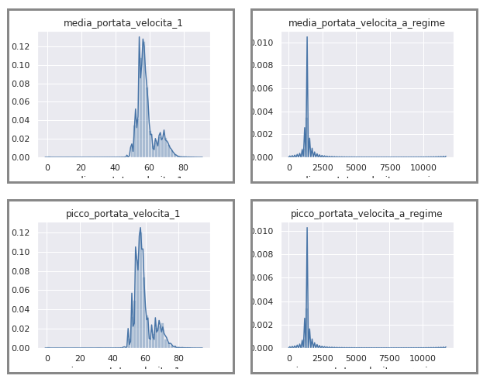
\includegraphics[width=1 \linewidth]{port.png}
    \label{fig:em}
    \caption{Distribuzioni delle grandezze relative alla portata.}
\end{figure}
{\begin{table}[h]
\centering
\begin{tabular}[t]{lccc}
\toprule
Portata&Minimo&Media&Massimo\\
\midrule
\textbf{Picco (140)}&30.30&58.96&93.6\\
\textbf{Picco (2300)}&930.5&1309.6&1422.9\\
\textbf{Media (140)}&28.07&58.5&90\\
\textbf{Media (2300)}&927.63&1304.8&1416.2\\
\bottomrule
\end{tabular}
\caption{Rassunto relativo alla media e al range dei valori di portata.}
\end{table}}
I comportamenti mostrati dalle osservazioni relative alla pressione della pompa si ritrovano in forma identica esaminando le misurazioni di portata: anche qui, esiste una grandissima somiglianza fra le distribuzioni di picco e media, e - come anticipato - una differenza di scala ancor più ampia fra i valori estratti per le due velocità (Figura 7).
\begin{figure}[h]
    \centering
    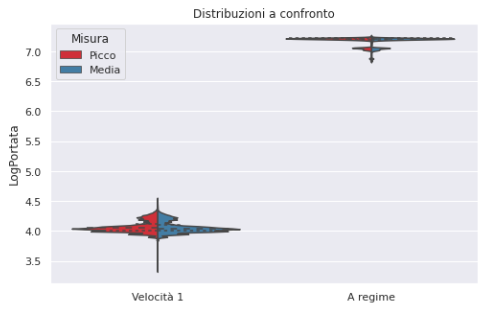
\includegraphics[width=1 \linewidth]{port2.png}
    \label{fig:em}
    \caption{Distribuzioni delle grandezze relative alla portata, in corrispondenza della velocità "1" e a regime, appaiate nell'ambito della stessa misurazione. Poichè la differenza era troppo grande per permettere una visualizzazione comprensibile, è stato necessario adottare una scala logaritmica.}
\end{figure}
\\
Infine, è interessante notare come le colonne relative alla pressione e alla portata condividano dipendenze lineari con grado molto elevato, come visibile in Figura 8: la correlazione assoluta media raggiunge addirittura un livello di $\sim$0.95, con un minimo di 0.79 - tra i picchi di portata misurati fra le due velocità - e 8 collinearità perfette. In particolare, oltre alla quasi identicità delle distribuzioni nell'ambito della stessa grandezza - menzionata in precedenza -, appaiono interessanti le seguenti dipendenze lineari:
\begin{itemize}
    \item picco pressione e picco portata, entrambi alla velocità di 140 \textit{r.p.m.} ($\sim$0.91)
    \item media pressione e picco portata, sempre per quanto riguarda la fase di controllo ($\sim$0.91)
    \item media portata e picco pressione, a 140 \textit{r.p.m.} ($\sim$0.92)
    \item media portata e media pressione, per la fase di controllo ($\sim$0.92)
    \item media pressione e media portata a velocità di regime, fra cui s'individua una correlazione perfetta
    \item picco pressione e picco portata a velocità di regime, sempre una correlazione perfetta
    \item picco portata e media pressione a velocità di regime: perfetta collinearità.
\end{itemize}
\begin{figure}[h]
    \centering
    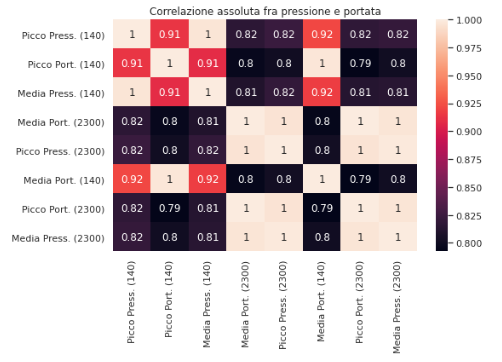
\includegraphics[width=1 \linewidth]{corrpp.png}
    \label{fig:em}
    \caption{Matrice di correlazione, con valori assoluti, fra tutte le variabili di pressione e portata.}
\end{figure}
Appare quindi evidente la sistematica dipendenza fra pressione e portata, che, osservando i dati forniti, paiono spesso essere state generate dalla stessa distribuzione casuale, a prescindere dalla misura scelta e dalla fase impostata. Per questa ragione, in fase di generazione dei modelli di regressione, la matrice del disegno potrebbe essere affetta da un eccessivo problema di multicollinearità, rischiando di divenire quasi-singolare o addirittura non invertibile, penalizzando una stima corretta sia dei coefficienti di regressione che degli indici di bontà di adattamento della funzione di regressione. Sarà pertanto necessario rimuovere tali variabili più correlate, oppure adottare strategie utili alla selezione di un modello a più bassa dimensionalità, come, ad esempio, le tipologie \textit{Ridge} e \textit{LASSO}.
\subsubsection{Altre variabili}
Le altre colonne numeriche, filtrate dalla fase di \textit{pre-processing} e ritenute rilevanti ai fini dello studio, sono: media coppia in fase finale (100 \textit{rpm}), picco coppia in fase finale e temperatura di prova del liquido.\\
Per quanto riguarda la prima, la distribuzione è fortemente asimmetrica verso valori elevati, con una discreta porzione di \textit{outliers}. Il picco della stessa grandezza presenta una coda ancor più lunga (in scala logaritmica in Figura 9). Medesima condizione di elevata asimmetria vale per la temperatura, compresa fra un range di $37.61^°$ e $49.1^°$.
\begin{figure}[h]
    \centering
    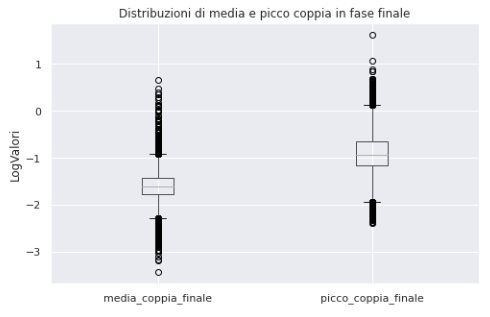
\includegraphics[width=1 \linewidth]{cf.png}
    \label{fig:em}
    \caption{\textit{Boxplot} per la visualizzazione della distribuzione delle variabili "Media coppia finale" e "Picco coppia finale".}
\end{figure}
È importante citare che anche fra la media e il picco della coppia in fase finale (100 \textit{rpm}) esista una forte dipendenza lineare positiva ($\sim$0.83). Bisognerà pertanto valutare questa ulteriore collinearità in fase di stima del modello per la previsione del coefficiente.\\
Al contrario, queste due variabili non presentano un'elevata dipendenza rispetto i dati di pressione e portata: la correlazione rimane sempre ben al di sotto del 20\%. Lo stesso vale per i valori di temperatura.

\subsection{Target: coefficiente di dispersione}
Il coefficiente di dispersione è calcolato con la formula
\begin{equation}\label{eq}
    \alpha=\frac{108.36-\text{Media portata (@140)}}{\text{Media pressione (@140)}}
\end{equation}
e i valori sono compresi in un range molto ampio, fra un minimo di $\sim$5.7 e un massimo di $\sim$817, con media e mediana rispettivamente pari a $\sim$27.8 e $\sim$29.43. La distribuzione è sbilanciata verso alti valori, come visibile in Figura 10.
\begin{figure}[h]
    \centering
    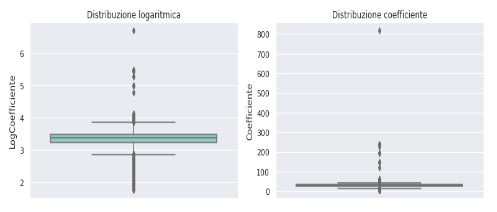
\includegraphics[height=100,width=1 \linewidth]{coeff.png}
    \label{fig:em}
    \caption{Distribuzione del coefficiente di \textit{leakage} in scala logaritmica e originale.}
\end{figure}
In Figura, è possibile notare una certa concentrazione dei \textit{records} in un intervallo di ampiezza ridotta attorno alla mediana. Questa considerazione è appurata dal basso coefficiente di variazione: $\sim$0.26.\\
Poiché il coefficiente di \textit{leakage} è indice della performance della pompa prodotta, è ragionevole supporre che ad ogni classe GP5, come conseguenza della differenza fra le proprie caratteristiche di progettazione e quelle delle altre categorie, si associ un diverso livello di prestazione - quindi un diverso \textit{range} di $\alpha$. Da un'analisi grafica superficiale (Figura 11), questa assunzione appare corretta: le distribuzioni del coefficiente, raggruppate per "Programma", appaiono spesso distanti, facendo ipotizzare l'esistenza di una notevole variabilità fra i gruppi, potenzialmente interessante per la costruzione di un modello predittivo. 
\begin{figure}[h]
    \centering
    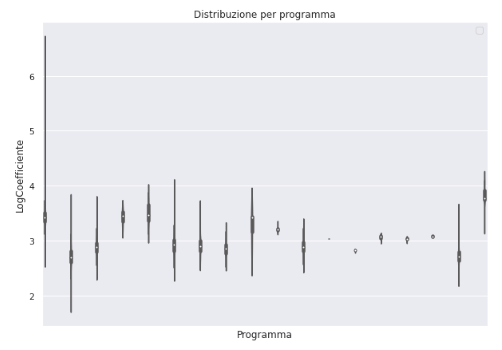
\includegraphics[width=1 \linewidth]{Programma.png}
    \label{fig:em}
    \caption{Distribuzioni del coefficiente $\alpha$ raggruppate per classe GP5 ("Programma").}
\end{figure}
Inoltre, è possibile che tale varianza fra le classi GP5 si manifesti non solo fra i livelli di performance, ma anche fra i coefficienti di regressione delle variabili esplicative scelte. In altre parole, è probabile che la selezione di un determinato Programma comporti una relazione significativamente diversa - rispetto agli altri tipi di pompe - fra $\alpha$ e le altre grandezze. Se questa ipotesi venisse verificata, allora si potrebbe dimostrare quanto il contributo delle varie parti coinvolte nel processo - monitorate attraverso la misurazione dei valori registrati nelle colonne nel database - si modifichi, influenzato dagli specifici fattori contestuali relativi alla diversa progettazione di ogni classe di pompa. In questo modo, sarebbe anche possibile ottimizzare il valore del coefficiente $\alpha$, monitorando questi fattori in maniera differente a seconda del Programma. Pertanto, con lo scopo di analizzare in maniera più approfondita la variabilità della funzione di regressione lineare di $\alpha$ in base al tipo di pompa in produzione, si è scelto di stimare una tipologia di modello misto adatta ai dati influenzati da effetti contestuali: il cosiddetto \textit{multilevel model}. Tale approfondimento è trattato nella Sezione \ref{Mod}.\\
Oltre alla relazione con "Programma", il coefficiente di dispersione mostra un collinearità molto elevata con molte altre colonne. Tralasciando le distribuzioni da cui $\alpha$ è stato generato (equazione \ref{eq}), le variabili con cui è più fortemente correlato sono relative alla pressione a regime ("Picco pressione velocita a regime" al 75\% e "Media pressione velocita a regime" al 74.6\%) e al picco di portata durante la stessa fase (74\%). Normalmente, queste dovrebbero essere quindi incluse nel \textit{subset} dei candidati esplicativi per la regressione lineare di $\alpha$, poiché potrebbero contribuire ad una stima accurata. Tuttavia, come si vedrà nella Sezione \ref{Mod}, la \textit{feature selection} sarà un'operazione difficile, a causa della multicollinearità rilevata fra le misurazioni di portata e pressione - in entrambe le fasi - e del conseguente rischio di ottenere una matrice del disegno quasi-singolare o invertibile. Ad esempio, se si volessero includere entrambe le variabili di pressione in fase di regime, la penalizzazione alla correttezza del modello non deriverebbe soltanto dalla loro reciproca collinearità, bensì anche dalla loro dipendenza lineare con le colonne utilizzate per calcolare $\alpha$.\\
La correlazione mostrata da $\alpha$ rispetto a "Media coppia finale" appare moderata (16.9\%), e "Picco coppia finale" ha una dipendenza lineare pari a circa il 7\%. È necessario ricordare che anche fra queste due grandezze esiste una collinearità rischiosa, la quale, nel caso in cui esse venissero incluse assieme nel modello, finirebbe per distorcere i coefficienti di regressione. Infine, la correlazione rispetto alla temperatura è ridotta: -6.9\%.\\
In seguito, poiché le osservazioni erano corredate da dati temporali relativi alla data - giorno, mese e anno - e all'orario, si è proceduto a verificare la possibilità di estrarre eventuali trend temporali. Tuttavia, le misurazioni appaiono cronologicamente disomogenee su due livelli. Innanzitutto, i \textit{record} nono sono stati forniti con coerenza temporale per quanto riguarda l'anno (Figura 12). 
\begin{figure}[h]
    \centering
    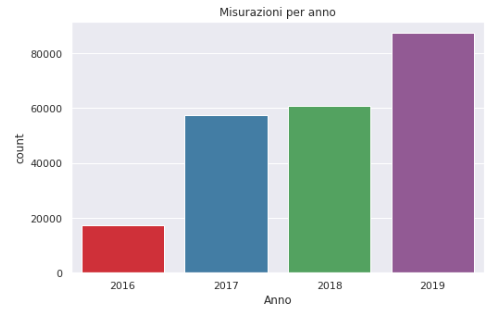
\includegraphics[width=1 \linewidth]{anno.png}
    \label{fig:em}
    \caption{Frequenza delle misurazioni per anno. I dati non sono stati forniti in maniera omogenea.}
\end{figure}
In ogni caso, non è comunque visibile alcuna differenza significativa fra le distribuzioni della performance nei vari anni (Figura 13).
\begin{figure}[h]
    \centering
    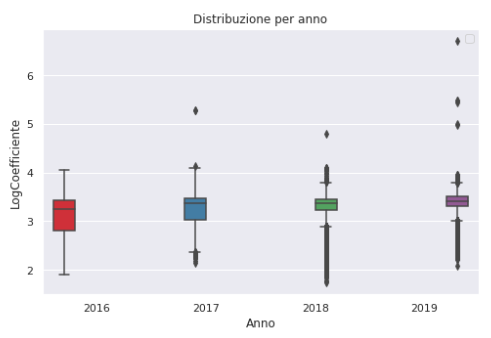
\includegraphics[width=1 \linewidth]{anno1.png}
    \label{fig:em}
    \caption{Distribuzioni del coefficiente $\alpha$ raggruppate per anno.}
\end{figure}
\\
Neppure per quanto riguarda il mese, le registrazioni sono omogenee, come visibile in Figura 14.
\begin{figure}[h]
    \centering
    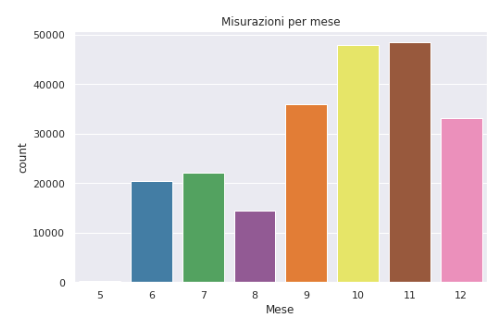
\includegraphics[width=1 \linewidth]{mese.png}
    \label{fig:em}
    \caption{Frequenza delle misurazioni per mese. I dati non solo non sono stati forniti in maniera omogenea, ma i primi 4 mesi sono addirittura mancanti, e maggio non riporta quasi osservazioni.}
\end{figure}
\\
Eppure, nonostante dalla collezione dei dati possa sembrare impossibile estrarre una certa periodicità per i motivi appena spiegati, l'andamento del coefficiente di dispersione è inaspettatamente armonico (Figura 15).
\begin{figure}[h]
    \centering
    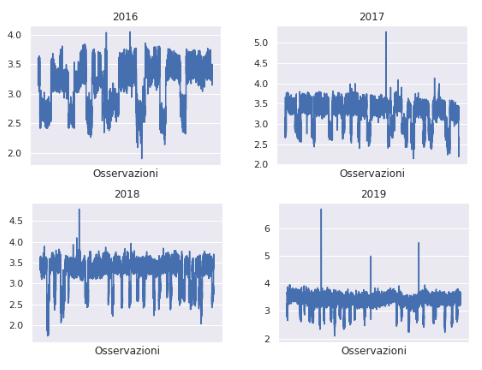
\includegraphics[width=1 \linewidth]{anni.png}
    \label{fig:em}
    \caption{Andamento del coefficiente di dispersione $\alpha$ per anno.}
\end{figure}
Tuttavia, è sufficiente eseguire un clustering grafico dei punti in base al programma di appartenenza per dedurre la motivazione di tale apparente periodicità: essa non deriva da un'autocorrelazione temporale fra i valori del coefficiente, bensì dall'ordine con cui è stato scelto di effettuare le misurazioni sui diversi gruppi GP5, che, come si è visto in precedenza, hanno distribuzioni differenti. L'andamento, perciò, appare generato da una sinusoide solamente perché le osservazioni alternano classi di pompa con performance elevate a categorie con un $\alpha$ minore. Quanto detto è evidente in Figura 16.
\begin{figure}[h]
    \centering
    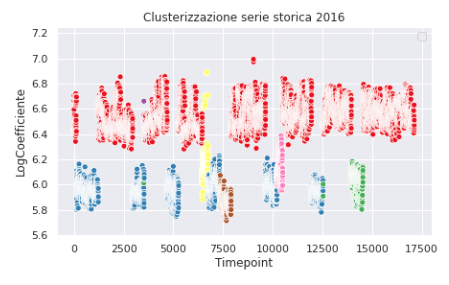
\includegraphics[width=1 \linewidth]{Cluster.png}
    \label{fig:em}
    \caption{Andamento del coefficiente di dispersione $\alpha$ durante l'anno 2016, clusterizzato in base alla variabile "Programma". Il colore rosso indica la tiplogia di pompa \textit{Daimler} - la più popolosa -, mentre gli altri colori sono associati alle sottocategorie Standard.}
\end{figure}

\subsection{\textit{Outliers Detection}}
L'ultima fase di analisi preliminare consiste nell'identificazione degli \textit{outliers}. Grazie ad essa, è possibile, in una fase di ottimizzazione della produzione, ricostruire il trend del processo, individuare le anomalie non segnalate dalla variabile "Esito" ed inferire eventuali fattori in grado di causarle. Innanzitutto, si è proceduto ad estrarre gli \textit{outliers} univariati all'interno della distribuzione del coefficiente di dispersione $\alpha$. Per farlo, poichè è stato verificato che tale distribuzione non fosse di tipo Normale, è stato applicato il metodo non parametrico della distanza interquartile, segnalando pertanto i punti inferiori a k volte il primo quartile e superiori a k volte il terzo quartile, con $k = 1.5$. È stato appurato che queste anomalie non dipendono da un particolare programma\footnote{Le anomalie sono presenti sia in corrispondenza della categoria \textit{Daimler} sia Standard.}, né si verificano in particolari anni o mesi.
\begin{figure}[h]
    \centering
    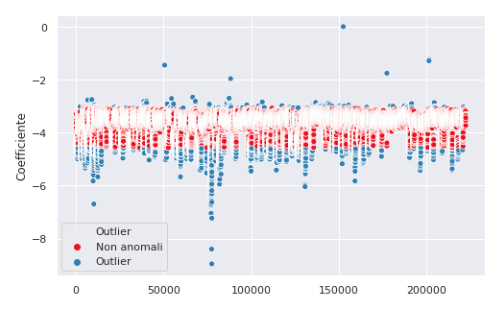
\includegraphics[width=1 \linewidth]{out.png}
    \label{fig:em}
    \caption{Identificazione degli outlier univariati all'interno della distribuzione del coefficiente di dispersione.}
\end{figure}
\\
Si è successivamente proceduto ad estrarre \textit{outlier} multivariati grazie all'algoritmo \textit{Local Outlier Factor} (LOF), basato sul calcolo delle deviazioni locali di ogni punto dal proprio vicinato. In questo caso, i valori anomali individuati rappresentano un porzione molto grande del database (75\%) e prescindono, come in precedenza, da particolari condizioni o programmi. Questa elevata quantità può dipendere dall'incidenza che gli specifici fattori contestuali di progettazione hanno sulle varie distribuzioni, elevando il grado di variabilità nell'andamento globale, così come dall'alternanza di fasi diverse nel processo. Sarebbe pertanto più utile applicare l'algoritmo di \textit{anomaly detection} separatamente in corrispondenza della cosiddetta velocità 1 (140rpm) e della fase di regime, e su ciascuna classe GP5.
%------------------------------------------------
\section{Sistema di monitoraggio \textit{real-time}}
Il processo industriale può essere ottimizzato grazie all'implementazione di sistemi di monitoraggio che individuino in tempo reale le eventuali anomalie, registrino i dati e li rappresentino graficamente su schermo per ottenere una visualizzazione \textit{user-friendly} dell'andamento delle variabili rilevanti. Nell'ambito di questo progetto, viene proposta una soluzione in grado di eseguire automaticamente le attività elencate. Tale sistema è stato interamente scritto e testato all'interno dell'ambiente di programmazione \texttt{Python}\footnote{Il codice è disponibile al seguente link: \url{https://github.com/RCrvro/Industry-Lab---Progetto/tree/master/Monitoraggio\%20realtime}.}.\\
Il programma, dunque, consta di tre elementi principali. Innanzitutto, si ha una componente di \textit{data ingestion}, la quale permette di ricevere il flusso di dati osservati dai sensori durante il processo di creazione di ogni pompa, ed elaborarlo per due scopi separati:
    \begin{itemize}
        \item rendere i dati adatti alla proiezione grafica sullo schermo;
        \item registrare metadati relativi alle misurazioni ricevute, \textit{timestamp} e valore decodificato, e segnalare se tale dato consiste in un \textit{outlier} univariato, aggiornando ad ogni \textit{step} il calcolo del metodo della distanza interquartile. 
    \end{itemize}
Questa operazione è stata simulata attraverso il client del \textit{software} \texttt{Apache Kafka}\footnote{Documentazione ufficiale del client di \texttt{Apache Kafka} in \texttt{Python}: \url{https://pypi.org/project/kafka-python/}.}, che si presta perfettamente al \textit{task} definito: si configura, infatti, come una piattaforma \textit{open source} a bassissima latenza per la gestione di \textit{feed} in tempo reale. Grazie al suo utilizzo, il sistema è in grado di ricevere grandi moli di osservazioni in intervalli di tempo molto ridotti, effettuare le elaborazioni prima citate ad altissima velocità e visualizzare il risultato grafico senza dover ritardare o ricaricare l'applicazione, e senza che l'utente debba controllare le operazioni in \textit{background}. Nel dettaglio, il sensore invia le misurazioni attraverso un \texttt{Producer} di \texttt{Apache Kafka}, e il sistema, connettendosi a un \texttt{Consumer}, effettua una lettura continua di questi dati all'interno del \textit{topic} in cui sono stati memorizzati. La lettura di un nuovo valore comporta, poi, l'estrazione dei metadati. Ad ogni sensore verrà applicato un \texttt{Producer} diverso, e per ciascuno verrà aperta una connessione verso il sistema tramite un \texttt{Consumer} separato, in modo da mantenere le letture indipendenti ed evitare un sovraccarico.\\
Il secondo elemento consiste in una componente grafica, curata mediante i \textit{tool} di visualizzazione forniti dall'interfaccia \texttt{Dash} di \texttt{Plotly}\footnote{Documentazione ufficiale di \texttt{Dash}: \url{https://plotly.com/dash/}.}. Essa riceve i valori letti dalla \textit{topic} di \texttt{Apache Kafka} e aggiorna in tempo reale due tipologie di visualizzazione per i dati inviati dai sensori: un \textit{BoxPlot} per monitorare la distribuzione totale, e un grafico \textit{LineChart} per l'andamento.\\
Infine, la terza componente - nominata "\texttt{writer}"\footnote{Il codice del "\texttt{writer}" è disponibile al link: \url{https://github.com/RCrvro/Industry-Lab---Progetto/blob/master/Monitoraggio\%20realtime/writer.py}.} - esegue un programma indipendente, che registra i metadati - \textit{timestamp}, dato numerico e segnalazione di eventuali valori anomali - all'interno di un database locale. Quest'ultimo, dunque, svolgerà la funzione di \textit{logfile} del processo. 
\subsection{Demo}
È disponibile una demo del sistema di monitoraggio al link \href{https://youtu.be/R7GCE91WyMc}{\textbf{\texttt{youtu.be/R7GCE91WyMc}}}. 
\\
In questo caso, si è scelto di simulare la visualizzazione di ipotetiche osservazioni relative al coefficiente di dispersione $\alpha$ (in verde) e alla media di portata a 140rpm (in arancione), perché, essendo variabile soggetta a limiti imposti in fase di produzione, appare ragionevole monitorarla in tempo reale.\\
Nel video, sul lato destro dello schermo, sono visibili quattro pagine del terminale. La prima in alto esegue un \texttt{Producer} per simulare l'invio delle misurazioni del coefficiente $\alpha$ da parte del proprio sensore, tramite scrittura manuale di alcuni valori. La seconda attiva un secondo \texttt{Producer}, per simulare il sensore della variabile di portata. La terza implementa il programma \texttt{writer}: ogni dato ricevuto dal sensore - in questo caso di $\alpha$ - viene scritto, assieme ai metadati, nel \textit{logfile} \texttt{"Coefficiente.csv"} apparso sul bordo destro del monitor dopo l'invio del primo valore. Alla fine del video, il file verrà aperto, per mostrare il risultato delle registrazioni. Inoltre, sempre per quanto concerne il \texttt{writer}, la pagina mostrerà un conteggio dei messaggi ricevuti. Infine, l'ultima finestra in basso inizializza l'applicazione grafica in corrispondenza della porta \texttt{8050} e mantiene connesso il sistema di monitoraggio.\\
L'applicazione è programmata per la segnalazione di eventuali errori, che possono essere esaminati cliccando l'icona blu nell'angolo inferiore destro della pagina \textit{Web}. 
%------------------------------------------------
\section{Limite dinamico di portata}
%----------------------------------------------------------------------------------------
\section{Modelli di previsione}\label{Mod}
%----------------------------------------------------------------------------------------
%	REFERENCE LIST
%----------------------------------------------------------------------------------------
\phantomsection
\bibliographystyle{unsrt}
\bibliography{sample}

%----------------------------------------------------------------------------------------

\end{document}
